%%%%%%%%%%%%%%%%%%%%%%%%%%%%%%%%%%%%%%%%%%%%%%%%%%%%%%%%%%%%%%%%%%% 
%                                                                 %
%                            CHAPTER                              %
%                                                                 %
%%%%%%%%%%%%%%%%%%%%%%%%%%%%%%%%%%%%%%%%%%%%%%%%%%%%%%%%%%%%%%%%%%% 

\chapter{Introduction}

\section{Introduction}
Over the last few decades, biologists have made major steps in trying to understand life; animals, humans, and plants. Since the rise of DNA sequencing techniques, genomics has become an emerging field within biology. However, genomic applications are often very computationally demanding, due to the size of the involved datasets, for example when analyzing the 3 billion base pairs of the human genome.

One fundamental application in genomics is short read genome mapping, which attempts to locate a short read of DNA on the full genome. If enough of such short reads are mapped, some interesting results can be achieved. For example, if enough reads are mapped, we can extrapolate the full genome of the organism. Even the amount of reads in one place (referred to as the reading depth) can give useful information, e.g. the presence of a trisomy of chromosome-21 in Down syndrome patients.

\begin{figure}[H]
	\centering
	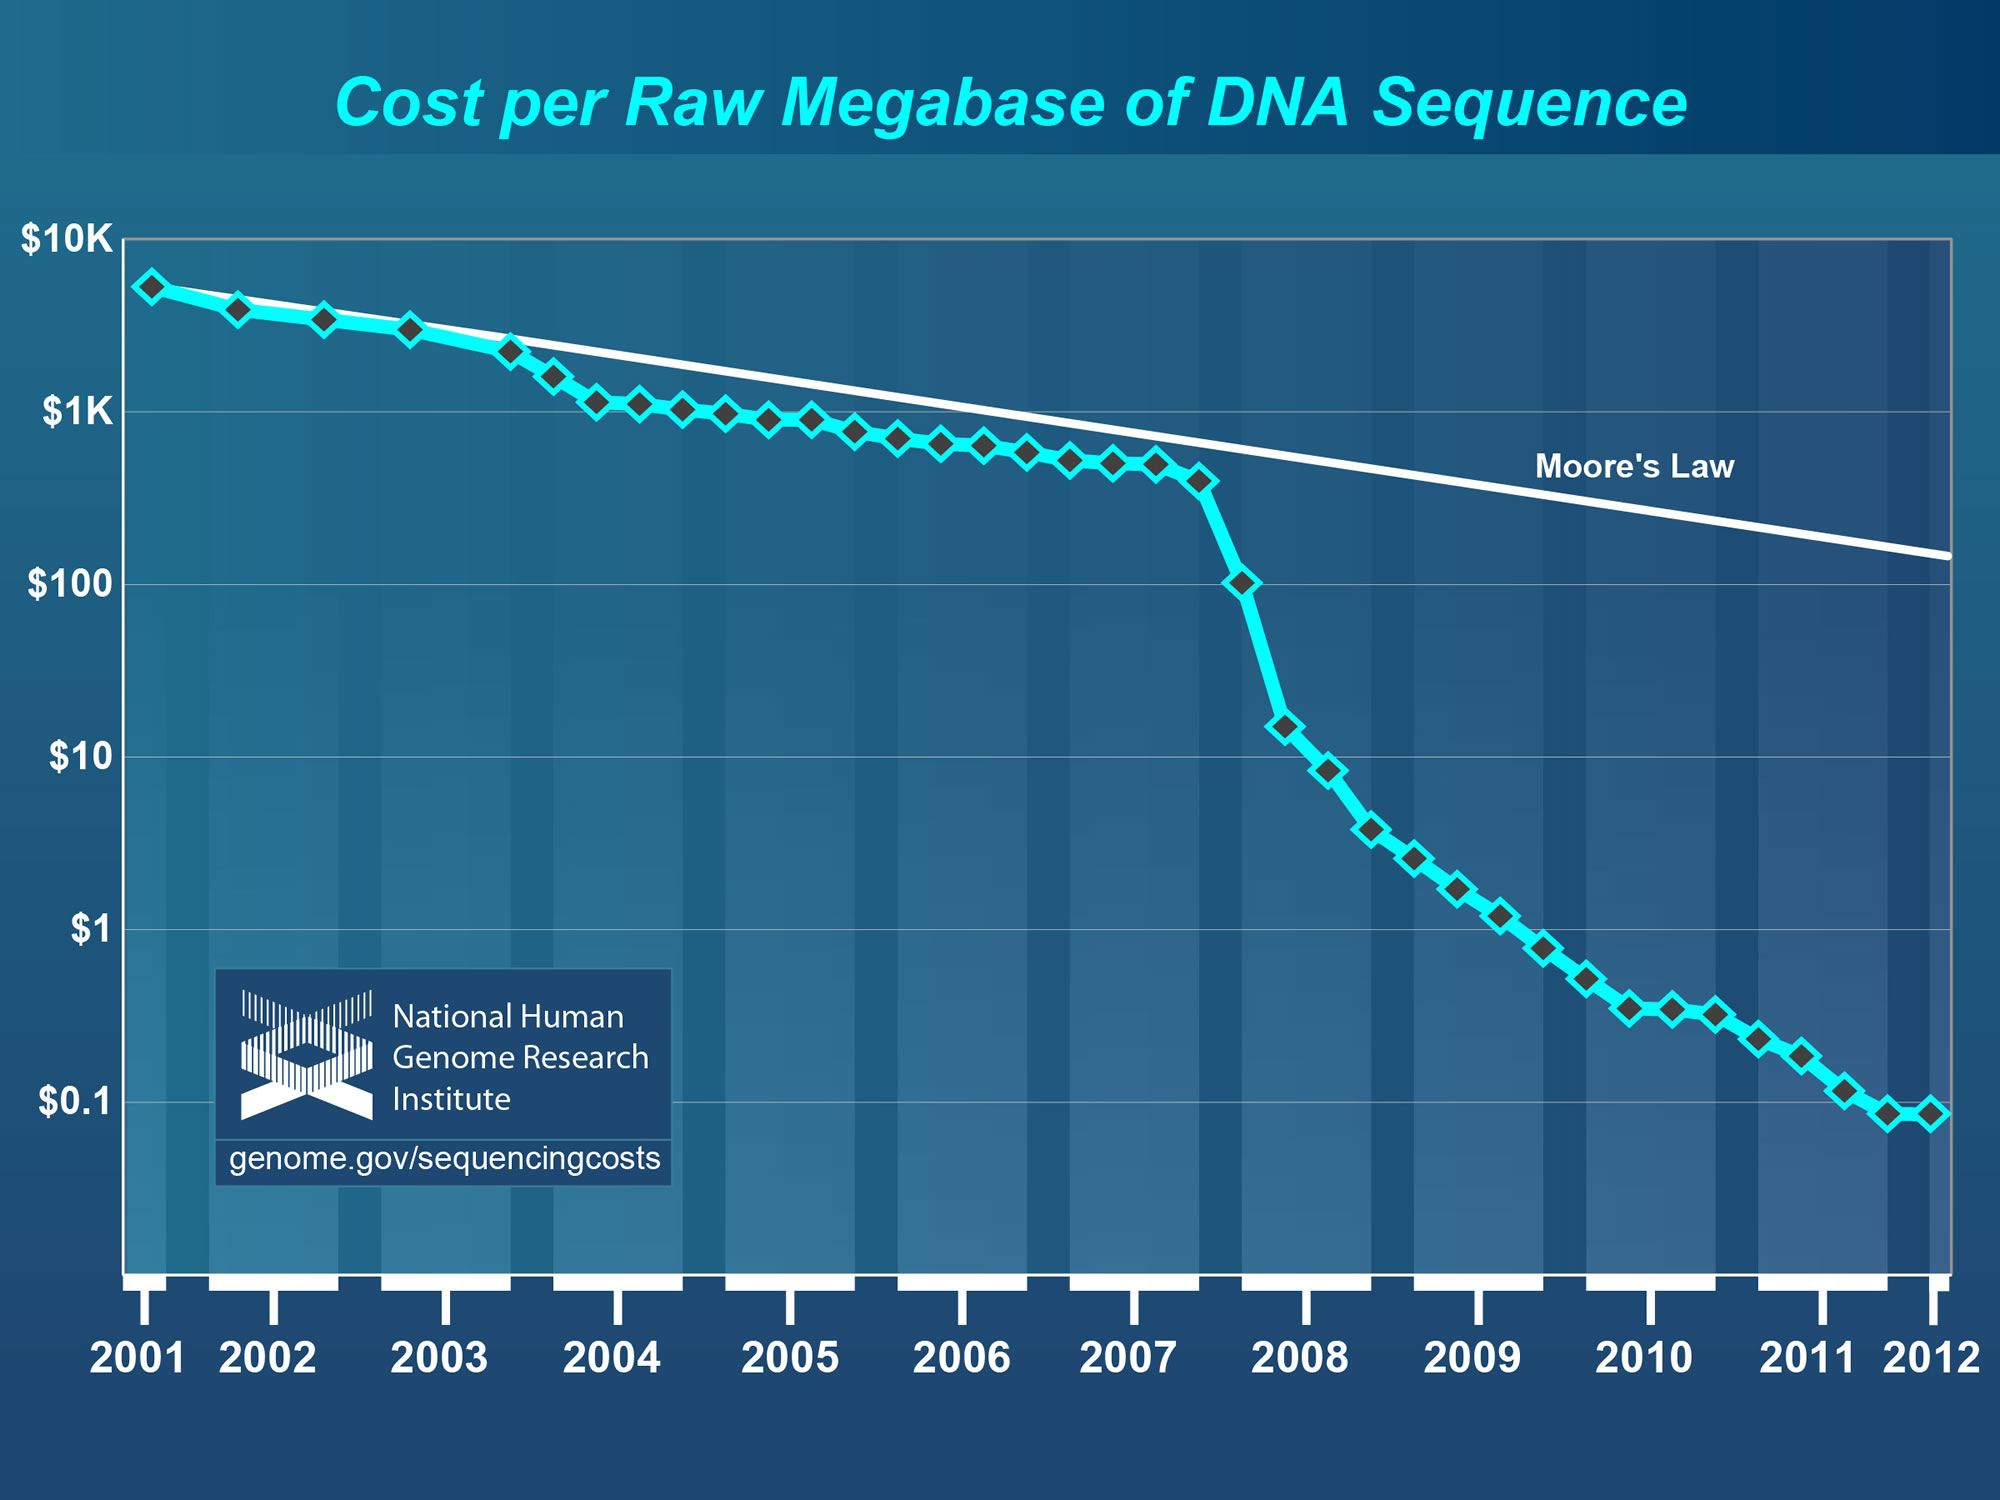
\includegraphics[width=0.5\textwidth]{introduction/costPerMegabase.jpg}
	\caption{Megabase means 1 million nucleotide bases. In this graph we can see that the cost of sequencing decreases significantly overtime, hence the demand of sequencing increases. This increases is more than Moore's law, which is the reason we that mapping techniques should improve to keep up with the demand~\cite{SeqCost}.}
	\label{fig:costMb}
\end{figure}

A full genome cannot be determined immediately, because the machines that determine this sequence can only handle short reads consisting of a few hundred bases. These sequencing machines are currently capable of producing millions of reads per day, and their throughput is growing at an exponential rate~\cite{SeqCost}. This exponential growth should be accompanied by an improvement in genome mapping techniques, to keep up with the throughput of these machines. However, most of the current software tools used for genome mapping are run on traditional CPUs. 

This thesis will implement genome mapping on an MPSoC (Multi-Processor System on Chip), which has an amount of programmable logic available to accelerate some aspects of the currently used algorithms. As a sample set, DNA sequencing reads of the PhiX and SARS-CoV-2 viruses will be explored. However, the algorithms discussed in this thesis can be expanded to the full human genome, where there is a high need for accelerating the algorithm and thus reducing the time-to-result of clinical tests.

\section{Organization of the chapters}

The further chapters of this thesis are organized as follows:

\paragraph{Chapter~\ref{ch:MBbackground}:} The theoretical background in genetics, molecular biology, and DNA, as well as the sequencing technology.
\paragraph{Chapter~\ref{ch:algoverzicht}:} The theoretical background regarding alignment, existing alignment algorithms, as well as the problem statement with some example clinical applications.
\paragraph{Chapter~\ref{ch:Platforms}:} The theoretical background on existing implementations of the Smith-Waterman algorithm on different kinds of hardware, as well as the hardware selection process.
\paragraph{Chapter~\ref{ch:InitDiff}:} A chapter which covers the difficulties I had when learning the required programming techniques, covering High-Level Synthesis and SDSoC. 
\paragraph{Chapter~\ref{ch:SoftwareImpl}:} A detailed description of the developed software implementation, as well as the results achieved with this implementation.
\paragraph{Chapter~\ref{ch:HardwareImpl}:} The analysis of the software implementation and where to accelerate using FPGA hardware. Also, the comparison between the accelerated version and the software version.
\paragraph{Chapter~\ref{ch:Conclusions}:} Conclusion and future work.